\documentclass[11pt]{article}

\usepackage{geometry}                % See geometry.pdf to learn the layout options. There are lots.
\geometry{letterpaper}                   % ... or a4paper or a5paper or ... 

\usepackage[parfill]{parskip}    % Activate to begin paragraphs with an empty line rather than an indent

\usepackage{amssymb}
\usepackage{epstopdf}
\usepackage{fixltx2e}
\usepackage{hyperref}
\usepackage{graphicx}
\DeclareGraphicsRule{.tif}{png}{.png}{`convert #1 `dirname #1`/`basename #1 .tif`.png}
\graphicspath{{./figures/}}

\begin{document}

\title{Diffusive Programming}
\author{Robert Philipp}
\date{\today}
\maketitle

%
% abstract
%
\begin{abstract}
This article describes an approach to task-oriented distributed programming that allows a developer to simply \emph{mark} a method to inform the distribution framework to distribute its execution. \emph{Diffusive programming} is defined through a set of principles that govern the action of distributing method-level execution and the topology of the distribution network. Through these principles, \emph{diffusive programming} allows the construction of distribution networks that can be tailored to solve specific or general problems,  learn/discover an optimal distribution network configuration for performing certain types of tasks, or that can contain sufficient redundancy to provide execution within required timelines. Finally, I describe \emph{Diffusive}, a reference implementation in Java, that meets the diffusive programming principles.
\end{abstract}

%
% introduction
%
\section{Introduction}
Task-oriented distributed computing allows independent computational tasks to be distributed to multiple computing nodes, presumably to execute in parallel. This approach can reduce the overall compute time of a set of independent tasks. For example, in quantitative finance, one may desire to calculate risk metrics on a large portfolio of financial instruments. Suppose that the calculation of these risk metrics for each instrument is independent of other instruments. In this case, we can speed up the calculation of the risk metrics for the entire portfolio by spreading these independent tasks over many compute nodes at once, and then collecting the results.

Typically this type of distribution is performed by a distribution middleware. In many cases, the application makes calls to the middleware's application programming interface (API) and implements an interface that represents a compute tasks. Including middleware API calls in the application code couples the application to the middleware. And more concerning, the application is now polluted with code used to distribute execution to remote compute nodes. Clearly, with careful design, much of the distribution logic can be hidden behind wrappers that allow the application logic to interact with an abstract compute engine which could execute locally or remotely. But even that approach doesn't overcome the constraints imposed by requiring that compute tasks implement a specific interface\footnote{An execution method is required. That means that any task must adhere to the signature of the execution method. And conversely, the signature of the execution method must be general enough to support any task.}.

Distribution middleware may also require deployment of certain resources (dynamic libraries, class files, etc) to the compute nodes \emph{before} they can execute remote requests. This requires careful synchronization of versioned resources. And this renders the compute nodes generic, only insofar as the required resources have been deployed to the node.

\emph{Diffusive programming} is an approach for performing task-oriented distributed computing that is based on the following principles intended to overcome challenges described above. In the remainder of this section I describe these principles and define some terms. In the next section, I discuss each principle in more detail. Note that the principles are ordered. The first two principles are related to the action of distributing execution, and the remaining principles are increasingly more focused on the configuration and topology of the compute nodes.

\begin{description}

	% marking, diffusive
	\item[Marking] 
	A method can be marked for remote execution. The act of \emph{marking}, alone, is sufficient and necessary for a method to be executed on a remote location and have the results returned. 
	
	\emph{Definition}: A \textbf{diffusive} method is a method that has been \emph{marked}.

	% location opaquenes
	\item[Location Opaqueness]
	Code calling a \emph{diffusive} method does not, and can not, know on which resource that method was executed. This helps keep code \emph{cohesive} by removing distribution logic from the application. 
	
	\emph{Definition}: A \textbf{diffused} method is a \emph{diffusive} method that was executed. 
	
	\emph{Definition}: A \textbf{diffuser} is what executes \emph{diffusive} method.
	
	% generic computation engine
	\item[Generic Computation]
	Any \emph{diffusive} method can be executed by a \emph{diffuser}. A \emph{diffuser} need not be configured with resources prior to requesting it to execute a method.
	
	% indistinguishablity
	\item[Indistinguishability]
	A \emph{diffuser} is responsible for executing any \emph{diffusive} method, and it is also responsible for \emph{diffusing} methods to other \emph{diffusers}. This implies that there is no distinction between workers and brokers, or clients and servers, in diffusive programming.
	
	% open topology
	\item[Open Topology]
	\emph{Diffusers} can be connected in any topology that can represented as a directed graph. Each node in the directed graph represents a \emph{diffuser}. Each directed edge represents a connection from one \emph{diffuser} to another. The direction of the edge represents the direction of the \emph{diffusion}. And, each \emph{diffuser} may contains connections to a set of other \emph{diffusers}. 
	
	\emph{Definition}: A \emph{diffuser network} is a set of connected \emph{diffusers}.
	
	\emph{Definition}: Suppose we have two \emph{diffusers}, \textbf{A} and \textbf{B}. We say that \textbf{B} is an \emph{end-point} of \textbf{A}, if \textbf{A} \emph{diffuses} methods to \textbf{B}.
	
	This principle allows the construction of networks tailored to solve specific or general problems, networks that can naturally learn/discover an optimal configuration for performing certain types of tasks, or networks that contain sufficient redundancy to provide execution within required timelines.

\end{description}

%
% Principles of diffusive programming
%
\section{Principles of Diffusive Programming}
In this section, I describe the five principles \emph{diffusive programming} in more detail. The principles build on each other, progressing from the action of distributing the code to the deployment and configuration of the \emph{diffusers}. I describe the reason for, and the importance of, each principle. Where applicable, I describe how the principle differs from more typical or traditional methods of distributed computing.

\subsection{Marking}
\emph{Diffusive programming} allows the execution of individual methods to be distributed. \emph{Marking} a method is the act of specifying that a specific method is to be distributed. How a method is \emph{marked} is up to the implementation of this principle. However, this principle does state that the act of \emph{marking} a method is necessary and sufficient for the method to be distributed. This means that \emph{any} method can be marked, and, therefore, executed, regardless of its name, parameters, or return type. This is a departure from many typical task-orient approaches that require the implementation of task interfaces, where the method to be executed has a defined signature (and return type).

The way a method is marked, to become a \emph{diffusive} method, depends on the implementation of this principle. For example, the reference implementation written in Java currently uses annotations to mark methods. However, it could just as easily allow the fully qualified method names to be specified in a configuration file instead.

The act of marking a method decouples the distribution logic from the application logic. And this leads us to the next principle: location opaqueness.

\subsection{Location Opaqueness}
\emph{Marking} a method tells the diffusive framework that that method is to be executed in a distributed manner. But it is the principle of \emph{location opaqueness} that places the requirement that any code calling a diffusive method does not know, or need to know, where that method is executed. Removing the responsibility of knowing or having to deal with the consequences of where the method is executed relieves the calling code of any responsibility regarding distribution. And this allows the application code to remain cohesive. It also means that the same code can be called in a distributed manner, or to run completely locally with any change to the application logic.

In typical distributed systems, the distribution logic must be called directly from the application code. This may occur by calling low level application programming interfaces (API) such as in MPI, or writing task classes that implement interfaces defined by the distribution framework, and then modifying application code to deliver these tasks to the middleware.

Location opaqueness allows code to be endowed with its execution logic, and that execution logic is then automatically mirrored, but in a distributed manner, simply by marking the method(s). When this is coupled with the next principle, \emph{generic computation}, we have a powerful and simple mechanism to distribute computation.

\subsection{Generic Computation}
The principle of \emph{generic computation} provides that any method can be executed on a \emph{diffuser} without out the need to deploy the resource needed to execute that diffused method. Simply put, the shared object libraries or classes don't need to be deployed to the remote server prior to making the request. Each \emph{diffuser} must contain a mechanism for providing resources to remote locations and for loading resources from a remote location.

In typical distributed computing, required resources must be deployed to the remote servers prior to requesting remote execution of a specific task. Diffusive programming removes this restriction by requiring that the mechanism which distributes the method execution also provides a capability to deliver the required resources to execute the method. 

Note that, however, this does not prevent users from deploying resources to a common location from which they can be obtained at run-time. Under certain deployment scenarios, it may be desirable to have such a common location to provide a centralized control over the versions. But even in this case, the resources need only be deployed to the one common area.

\subsection{Indistinguishability}
The principle of \emph{indistinguishability} means that a \emph{diffuser} must be able to receive requests to execute, and at the same time be able to \emph{diffuse} (forward) those requests to another \emph{diffuser}. In other words, there isn't such a thing as a client diffuser and a server diffuser: they are one and the same.

The \emph{generic computation} principle alluded to this principle of \emph{indistinguishability}. The generic computation principle states that a diffuser must be able to load resources from a remote diffusers, \textbf{and} at the same time must be able to provide resources to a remote diffuser.

\subsection{Open Topology}
The \emph{open topology} principle, coupled with the \emph{indistinguishability} principle, requires that it is possible to create networks of \emph{diffusers}, called \emph{diffuser networks}, in any topology that can be represented as a directed graph. Each node in the directed graph represents a \emph{diffuser}, and each (directed) edge connects that \emph{diffuser} to an \emph{end-point}, which is another \emph{diffuser}. Any network that can be represented by a directed graph can be constructed. Section \ref{sec:diffusion_patterns}, \nameref{sec:diffusion_patterns}, describes a few possible network topologies (patterns) that are designed to solve specific problems.

%
% Diffusion patterns
%
\section{Diffusion Patterns}\label{sec:diffusion_patterns}
\emph{Diffusion patterns} are made possible by the last three diffusive programming principles: generic computing; indistinguishability, and open topology. Together, these three principles make the statement that \emph{diffusers} form building blocks that can be connected as directed graphs. The principle of \emph{open topology} requires that a diffuser be connected to zero or more end-points to which it can diffuse execution of a method. The principle of \emph{indistinguishability} states that each end-point, itself, must be a diffuser. This means that that diffuser itself is connected to zero or more other end-points. And, therefore, it can receive tasks as well as diffuse them. Finally, the principle of \emph{generic computing} requires that a diffuser be able to receive (and send) resources needed to execute a task, allowing tasks to be diffused to other nodes dynamically and executed.

Because any diffuser network that can be represented as a directed graph is possible to construct, there are an infinite number of patters in which these networks can be constructed. And furthermore, their dynamic nature also allows the networks to evolve over time. In the next subsections I describe three illustrative patterns that solve specific problems.

Finally, it is important to emphasize that it is the \emph{marking} principle and the \emph{location opaqueness} principle that require the diffusive framework to provide a mechism for intercepting \emph{marked} method calls and handing them to the (local) diffuser assigned to the application. It is that (local) diffuser that then takes care of diffusing the execution of the \emph{marked} method to other remote diffusers for execution. Therefore, all the topologies have this characteristic in common.

% layer network topology
\subsection{Layered}
The layered topology is the simplest, and most similar to many distributed middleware solutions. In this topology, the diffuser collocated with the application, which we will call the \emph{application-attached diffuser}, is connected to a set of end-points, which we call the \emph{remote diffusers}. The application-attached diffuser, depending on the specifics of its configuration, is responsible for distributing the tasks to the the remote diffusers. The remote diffusers execute the task and return the results to the application-attached diffuser, which returns the results to the application\footnote{In the discussion about the reference implementation, \emph{Diffusive}, I'll provide details on how these steps can be implemented.}. 

Figure \ref{fig:topology_single_layer} shows the simplest topology---a single layered diffuser network. In this figure, the circles label with \textbf{D} are \emph{diffusers}, the square at the bottom label with \textbf{A} is the application containing the methods to be diffused. In this topology, the application-attached diffuser is responsible for distributing the tasks to the remote diffusers. The remote diffusers execute their assigned task and return the result to the application-attached diffuser, which then returns it to the application.

\begin{figure}[htbp]
\begin{center}
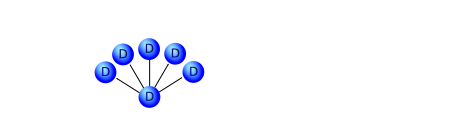
\includegraphics[scale=1.0]{topology_single_layer}
\caption{Single Layer Diffuser Network Topology\label{fig:topology_single_layer}}
\end{center}
\end{figure}

Although not covered in the diffusive principles, because it is an implementation detail, it is worth noting at this point that any implementation must address the strategy used to distribute the tasks amongst the diffusers---local and remote. The reference implementation \emph{Diffusive} provides a \textsf{Strategy} interface that can be implemented to provide a specific strategy based on load, number of executing threads, weighting, or some other scheme. Clearly, the implementation of such a strategy will effect the performance characteristics of the diffusive network.

A natural extension of the single-layered diffuser pattern is a multi-layered diffuser pattern. One such pattern is  shown in figure \ref{fig:topology_multi_layer}. If the implementation of the diffusive principles allows nested method \emph{marking}, this topology allows tasks to be diffused that, themselves, contain subtasks. One example where such a network topology would be far more suitable than a single layered topology is when the task, itself, is composed of multiple independent subtasks that each produce a large amount of data which the task combines. Allowing the diffusers in the first layer to perform the combining (averaging, summation, etc) before returning the result to the application-attached diffuser alleviates the application-attached diffuser from become overloaded with the tasks of combining a many large sets of data. 

\begin{figure}[htbp]
\begin{center}
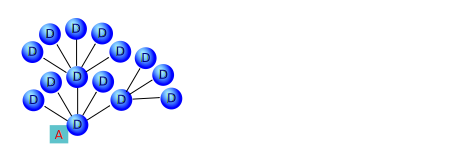
\includegraphics[scale=1.0]{topology_multi_layer}
\caption{Multi-Layer Diffuser Network Topologies\label{fig:topology_multi_layer}}
\end{center}
\end{figure}

This type of topology can dramatically improve the performance such calculations. However, this network topology is only an improvement \textbf{if} nested method marking is supported. In practice nested method marking is difficult to implement in a generic manner. In fact, it is not part of the reference implementation.

%The topology depicted on the left-hand side of the figure simply provides the diffusers in the first layer additional diffusers to which to diffuse tasks in the event that their load is too high. The utility of such a network is questionable because it would usually be more efficient to simply add the second-layer diffusers to the first layer. However, if the implementation of the diffusive principle allowed nested method \emph{marking} then such a network design could be used to distribute tasks that contained subtasks requiring post processing. However, in practice this is difficult to implement in a generic manner, and therefore, is not part of the reference implementation.

%The diffuser network on the right-hand side of figure \ref{fig:topology_multi_layer} is intended to provide a mechanism for load balancing. However, again, the appropriate diffusion strategy diffusing tasks to the same total number of diffusers should be more efficient. 

% redundant network topology
\subsection{Redundant}
In distributed computing it is not uncommon that a task fails to complete. A compute node may have crashed or lost network connectivity with the collective. Or some mysterious set of events placed the execution of the task in an unusual, never-to-be-repeated-until-a-demo state that prevented its completion. In cases where the completion of each individual task is required to occur at least once in a given time period, we could send redundant tasks to different compute nodes, and use the first result from each individual task to come back.

The principles of \emph{generic computation} and \emph{location opaqueness} mean the the implementation of the diffusive principles hides this from the application. The application configuration would be the only change to the application's execution. Furthermore, it turns out that this redundancy is quite straight forward to implement through the user of the \textsf{Strategy} interface. By having the \textsf{Strategy} return a set of endpoints, rather than a single one, the same tasks can be sent to all the end-points in a set. The first result to return is passed to the application, and the rest are either ignored, or cancelled.

\subsection{Learning}
Not all servers are created equal. For purposes of distributed computing, I focus on three important differences:
\begin{enumerate}
\item Execution capacity
\item File input-output (I/O) capacity
\item Network I/O capacity
\end{enumerate}

Execution capacity describes the available processing capacity of the server\footnote{I am referring to a physical server in these examples. However, the arguments apply equally as well if the servers are virtualized, but roughly guarantee a certain execution capacity.}. All else equal, servers with a higher processor and core count will provide higher execution capacity. Clearly there are many other factors that determine the execution capacity of a server. And, therefore, when distributing execution tasks, having information about the execution capacity of a server helps determine the optimal amount of work to distribute to that server relative to other servers. 

As an oversimplified example, suppose that you have two servers available to which tasks can be sent: server \textbf{A} and server \textbf{B}. If the server \textbf{A} has four processors and server \textbf{B} has only one processor, then if the servers are otherwise the same, you would expect  that server \textbf{A} can process about four times as much work as server \textbf{B}. If the tasks involve writing a large amount of data to a distributed data base, then it may be necessary to consider differences in the servers' file I/O or network I/O capacity when determining the optimal distribution of tasks.

To account for the differences in the capacity of a server to perform tasks, one can use a \textsf{Strategy} that takes in to account weighting factors assigned to each server. These weighting factors would be configured to represent the capacity of the node to perform specific sets of tasks. And the \textsf{Strategy} would select servers for tasks based on their weighting. For example, if server \textbf{A} had four processors and server \textbf{B} has only one processor, we may configure server \textbf{A}'s weight to be four, and server \textbf{B}'s weight to be 1. The \textsf{Strategy} would use these weights to send about for times as many tasks, on average, to server \textbf{A} than to the server \textbf{B}.

The assignment of these relative weights to each server can be automated in cases where the same type of processing is performed repeatedly. This type of automation can be achieved through the use of a \textsf{Strategy} that adjusts the weights and the logs them. Once the overall execution of the process is complete, the application-attached diffuser makes an associate of the overall execution time (possibly scaled to the number of similar tasks) with those weights. The next time the process is run, \textsf{Strategy} uses this information---weight-to-server assignments and the execution time of that combination---to again adjust the weighting factors according to some optimization algorithm.

%
% Reference implementation
%
\section{Diffusive: Reference Implementation}
The \emph{Diffusive} reference implementation is a Java-based framework that implements the \emph{diffusive} principles. Aspects of \emph{Diffusive} are specific to its implementation, and could be implemented in other ways. For example, in \emph{Diffusive} methods are \emph{marked} through the use of annotations. In particular, a \emph{diffusive} method is annotated with \textsf{@Diffusive}. However, it would have been possible to allow methods to be marked through a configuration file that holds a list of \emph{markers} represented by their fully qualified method names\footnote{For example, the fully qualified method name could be represented by the fully qualified class name with the method name appended with a ``.'', such as \textsf{org.myapp.calc.PriceCalc.calculate}.}. These aspects only change the specifics of how a \emph{diffusive} framework implements the principles, but not how it behaves.

In the next sections I discuss how \emph{Diffusive} framework implements the five diffusive principles.

% marking and diffusing
\subsection{Marking and Diffusing\label{sec:marking_and_diffusing}}
The diffusive principle, \emph{marking}, requires that a method is somehow identified as a \emph{diffusive method}. It further requires that \emph{marking} a method is both sufficient and necessary for a method to be diffused. The \emph{location opaqueness} principle takes it a step further by requiring that any application method calling a diffusive (marked) method does not, and can not, know where that method is being executed.

% launching and instrumentation
\subsubsection{Launching and Instrumenting\label{sec:launching_and_instrumenting}}
\emph{Diffusive} accomplishes this through a combination of annotations and load-time byte-code engineering. The annotations are simple: any method that is to be diffused is annotated with \textsf{@Diffusive}. This signals the class-loader that any calls to this method should be replaced with a call to a diffuser that has already been configured\footnote{I'll discuss the configuration of \emph{Diffusive} later.}. \emph{Diffusive} uses the byte-code engineering framework \href{http://www.jboss.org/javassist/}{Javassist}\footnote{\url{http://www.jboss.org/javassist/}}\textsuperscript{,}\footnote{Another approach would have been to use aspect-oriented programming frameworks such as AspectJ. However, the compact Javassist framework provides everything \emph{Diffusive} needs.} to replace marked method calls with calls to the diffuser instead and hands the diffuser information about the method call\footnote{Particularly, and at a minimum, the diffuser needs to know the name of the method, it's parameter types and values, its return type, and the name of the class that containing it.}.

In order to replace marked methods during class-loading, the application classes must be loaded through the diffusive class loader (\textsf{DiffusiveLoader}). This is accomplished by using an application launcher, called the diffusive launcher (\textsf{DiffusiveLauncher}). The diffusive launcher accepts the name of the application's Java class, creates a diffusive class loader, and asks it to run the application. The diffusive loader reads the configuration items, sets up the application-attached diffuser to which marked method calls are diverted, and determines whether a class is loaded by the application's class loader and which are passed to the Javassist \textsf{Loader}.

\begin{figure}[htbp]
\begin{center}
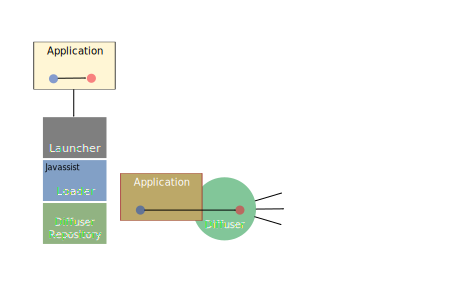
\includegraphics{diffusive_launcher}
\caption{Launching an application in Diffusive}
\label{fig:diffusive_launch_application}
\end{center}
\end{figure}

Figure \ref{fig:diffusive_launch_application} illustrates launching an application in \emph{Diffusive}. At the top of the figure is a box labeled ``Application'' which represents the unadulterated application. The light blue dot in that box represents a method call to the red dot. The red dot represents a \emph{marked} method. The application passes through the launcher and into the loader. The \textsf{DiffusiveLoader} sets up the repository holding the default diffuser, reads the configuration items, creates an \emph{application-attached} diffuser, and hands the application to the Javassist \textsf{Loader} to instrument the application. The tan box labeled ``Application'' in the lower-right hand side of the figure represents the instrumented, or modified, application. Notice that now, all the method calls to the \emph{marked} method are diverted to the \emph{application-attached} diffuser, which contains the required mechanism to execute that method. It is the application-attached diffuser, the green circle on the bottom left-hand side of the figure, that is responsible for distributing the method execution. It is important to point out that the original application code is untouched.

% distributing
\subsubsection{Distributing\label{sec:distributing}}
The \emph{application-attached} diffuser is responsible for executing for distributing method calls to other diffusers, or depending on its configuration and load, executing the method. By default \emph{Diffusive} uses a \emph{RESTful} diffuser (\textsf{RestfulDiffuser}) that adheres to the \href{http://jsr311.java.net}{JSR-311} standard\footnote{\url{http://jsr311.java.net}}, and the \href{http://jersey.java.net}{Apache Jersey}\footnote{\url{http://jersey.java.net}} implementation. Although \emph{Diffusive} uses a RESTful diffuser by default, any diffuser implementation can be used to provide the required functionality. In fact, \emph{Diffusive} also comes with a local diffuser that runs the code locally.

The RESTful diffuser must be configured with a set of \emph{end-points} to which it can diffuse method execution. These end-points, themselves, must contain a RESTful diffuser. And the access to the diffuser must be accomplished through a some sort of a software server. \emph{Diffusive} provides a RESTful diffuser server (\textsf{RestfulDiffuserServer}) that contains an \href{http://grizzly.java.net}{Apache Grizzly}\footnote{\url{http://grizzly.java.net}} web server configured to interact with a \href{http://docs.oracle.com/javaee/6/tutorial/doc/giepu.html}{JAX-RS}\footnote{JAX-RS implements JSR-311, providing an implementation for developing RESTful web services in Java. For more information, visit \url{http://docs.oracle.com/javaee/6/tutorial/doc/giepu.html}.} web resource (\textsf{RestfulDiffuserManagerResource}).

Within the context of the RESTful diffuser server, there is one RESTful diffuser for each diffusive method. In other words, each unique diffusive method signature\footnote{A diffusive method signature contains the name of the containing class, the method name, the method's formal argument types, and the return type. This is different from a Java signature, which contains only the method name and the formal argument types.} has its own diffuser, accessible via the web resource (\textsf{RestfulDiffuserManagerResource}) through its uniform resource identifier (URI). The web resource manages the creation, querying, calling, and deletion of its diffusers by responding to requests from the calling diffuser. And each diffuser is a resource with a unique address. For example, a new diffuser is create through an \texttt{HTTP POST} call containing the required information about the diffusive method signature. Obtaining information about a diffuser is obtained through an \texttt{HTTP GET} call to its URI. To execute a method, an \texttt{HTTP POST} is called on the URI of the diffuser, passing along the information needed to execute the method. The execute method returns an ID (link) to the results resource\footnote{Hypermedia as the engine of application state (HATEOAS).}. The result can then be obtained through an \texttt{HTTP GET} call to the URI of that result, which blocks until the result is complete. Alternatively, the status of the result can be obtained through an \texttt{HTTP HEAD} call to the URI of the result, which is non-blocking, and returns an empty response if the result resource is not yet available. And, finally, a diffuser can be deleted through an \texttt{HTTP DELETE} call to its URI.

% distribution strategy
\subsubsection{Distribution Strategy\label{sec:distribution_strategy}}
Diffusers decide how to distribute the method calls based on a strategy (\textsf{Strategy}). A \textsf{Strategy} simply returns a list of end-points with each request. In most cases, the list returned by the \textsf{Strategy} contains only one element. However, to allow for redundant diffuser networks, the \textsf{Strategy} interface allows the return of a list of end-points. \textsf{Strategy} implementations can take into account various aspects that affect the optimal distribution of method calls. For example, a \textsf{Strategy} implementation can take into account the load on its server, the number of diffusers executing, the number of threads available for execution, and weighting factors for individual end-points.

% serialization
\subsubsection{Serialization\label{sec:serialization}}
In order to execute a method remotely, the remote execution environment needs certain information. The execution environment needs:
\begin{enumerate}
\item The state of the object against which the method call was made. This state is equivalent to a serialization of the object tree: the object and all objects referenced by the object.
\item All the arguments to the method.
\end{enumerate}
And to move these objects across the wire, they need to be serialized. And once execution is completed, the return object must be serialized and returned to the original diffuser.

Once the execution environment receives the serialized objects, it needs to reconstruction them, and for that it needs the Java \textsf{Class} objects. The \textsf{Class} objects are effectively the templates used to reconstruct an object. In the next section we discuss how the remote environment gets access to these \textsf{Class} objects without a need to deploy them prior to execution.

\emph{Diffusive} provides an interface, \textsf{Serializer}, that defines what a serializer must provide to \emph{Diffusive}. Two key serialization implementations have been wrapped to conform to the \textsf{Serializer} interface: \textsf{ObjectSerializer} and \textsf{PersistenceSerializer}. The \textsf{ObjectSerializer} is Java's own serialization framework which requires that classes implement the \textsf{Serializable} interface. Using this serialization framework this requires altering existing classes that don't yet implement \textsf{Serializable}. In some cases this may be acceptable. In other cases it may not be possible.

The \textsf{PersistenceSerializer} wraps the \href{http://freezedried.sourceforge.net}{FreezeDry} persistence framework\footnote{\url{http://freezedried.sourceforge.net}}. FreezeDry does not require any classes to implement a FreezeDry-specific interface. In fact, FreezeDry can take any existing class (even those without no-arg constructors) and serialize them into XML, JSON, or key-value pairs. However, if the class is too complex, it may require some coding.

% generic computation
\subsection{Generic Computation\label{sec:generic_computation}}
Section \ref{sec:serialization}, \nameref{sec:serialization}, described the need for serializing objects for transport across the network, and for the remote diffuser to be able to execute the diffusive method. Recall that to execute a diffusive method requires the object containing the serialized method and all the objects passed as arguments to the method to be serialized. Once these serialized objects are received by the remote diffuser, it needs to deserialize them back into objects. To deserialize any object requires that the class loader has loaded a \textsf{Class} object corresponding to that object (and any objects that object references). Usually, this is handled by deploying the class files (as jar or war files) to the remote servers that will be executing the methods.

The \emph{Generic Computation} principle states that deployment of resources to the remote nodes must not be necessary. \emph{Diffusive} provides

%
% Future work
%
\section{Future Work}

%Before describing these principles and their implications in more detail, I illustrate how such an approach could behave. First you would create a \emph{diffuser network} by running \emph{diffusers} on a collection of servers. Then you would configure the \emph{diffuser network} by giving each \emph{diffuser} a set of \emph{end-points} to which it can \emph{diffuse} method execution. Then you would specify, through configuration, which methods should be diffused. Then you need to instrument the code so that when the specified methods are called, the method calls are intercepted, and diverted to a \emph{diffuser}, which executes the method and returns the result, or diffuses the method further.

%Although this may seem complicated, a framework constructed from the above principles, would only require that the \emph{diffusive} methods be specified, and the code could be launched through a container that would automatically instrumented the code to divert method calls. In this way, there isn't any need to modify the base code.

%I have developed an open-source reference implementation of a Diffusive framework in Java that meets the above principles. Through the use of Aspect-Oriented programming frameworks, one could also implement such a framework in C/C++.

%Suppose we needed to perform 800 calculations, each calculation tools about 1 minute to execute. Suppose further that we had written code to run on a dual-quad-core server. And, on this hardware it took about 2 hours to execute. Suddenly, we are given access to 100 similar servers and asked to distribute the calculation across these 100 servers to reduce the computation time to a few minutes.

%Task-oriented distributed computing is difficult. Endowing applications with the ability to execute tasks remotely, typically requires calls to an application programming interface (API) that manages the distribution of those tasks to remote servers. Typically, these servers must be configured to run the desired tasks.

%Coding to such an API pollutes the application's \emph{business} logic with its distribution logic. It is true that with care the business and distribution logic can be cleanly separated in most cases. However, when an application needs to provide the ability to execute its tasks both locally and in a distributed mode, applications will require two versions of the execution logic: one for running locally, and one for distributed execution.

%Embedding execution distribution code into the application, in any case, causes additional difficulties for testing the business logic and debugging. 

% reference impl�mentation
%This reference implementation allows developers to simply annotate methods whose execution is to be distributed. Then they launch the application through a \emph{diffusive launcher} that instruments the code at load-time, replacing the annotated method calls with ones that distributes the execution.

%\subsection{}



\end{document}  